\documentclass[english]{article}

%% Packages pull in extra commands:
%% http://en.wikibooks.org/wiki/LaTeX/Packages

\usepackage{hyperref}
\usepackage[letterpaper]{geometry}
\geometry{verbose,tmargin=1in,bmargin=1in,lmargin=1in,rmargin=1in}
\usepackage{amsmath}
\usepackage{amssymb}
\usepackage{graphicx}
\usepackage{float}
\usepackage{array}
\usepackage{tikz}
\usepackage{enumitem}

% New commands serve as shorthand for frequently used command combinations.
\newcommand{\ind}[1]{\mathbf{1}\left(#1\right)}
\newcommand{\bx}{\mathbf{x}}
\newcommand{\E}{\mathbf{E}}

\title{CIS 520, Machine Learning, Fall 2018: Assignment 2\\
Due: Sunday, September 23rd, 11:59pm (via turnin)}
\author{Wentao He}

\begin{document}
\maketitle

{\normalsize \noindent Collaborators: \underline{Ruo Jia}} \\

\section{Cross Validation}

For the code part, please see \path{make_xval_partition.m} in \textbf{turnin}.\\

\section{K if for Kernel Width}

For the code part, please see \path{k_nearest_neighbours.m}, \path{kernel_regression.m}, \path{knn_xval_error.m} and \path{kernreg_xval_error.m}.\\

\begin{enumerate}[label=(\roman*)]
    \item For both the original data and the noisy, compute both the $N$-fold error on the training set, for $N = \{3, 5, 9, 15\}$, and the test error for K-NN, and Kernel Regression with $K = 1$ and $\sigma = 1$ respectively.
    \begin{enumerate}
        \item Figure on original data with KNN.\\ \\
        Please see Figure \ref{fig:211}. \\
        \begin{figure}[H]
          \centering
          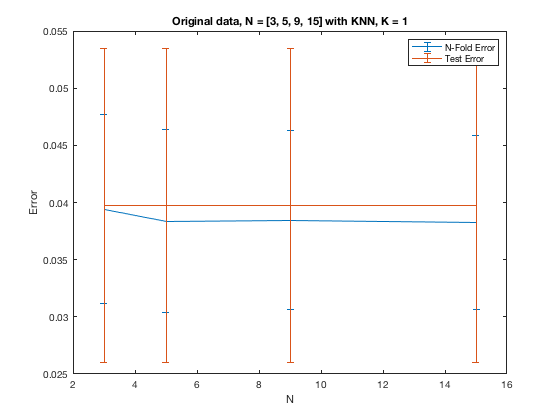
\includegraphics[width=0.6\textwidth]{211.png}
          \caption{Figure on original data with KNN.}
          \label{fig:211}
        \end{figure}
        \item Figure on noisy data with KNN.\\ \\
        Please see Figure \ref{fig:212}. \\
        \begin{figure}[H]
          \centering
          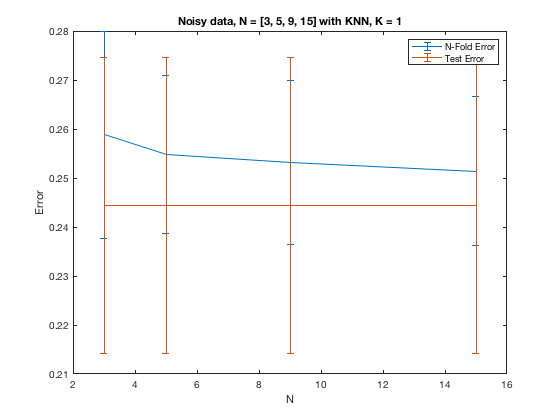
\includegraphics[width=0.6\textwidth]{212.png}
          \caption{Figure on noisy data with KNN.}
          \label{fig:212}
        \end{figure}
        \item Figure on original data with Kernel Regression.\\ \\
        Please see Figure \ref{fig:213}. \\
        \begin{figure}[H]
          \centering
          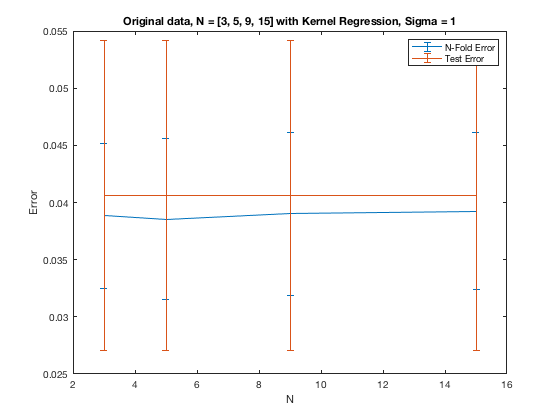
\includegraphics[width=0.6\textwidth]{213.png}
          \caption{Figure on original data with Kernel Regression.}
          \label{fig:213}
        \end{figure}
        \item Figure on noisy data with Kernel Regression.\\ \\
        Please see Figure \ref{fig:214}. \\
        \begin{figure}[H]
          \centering
          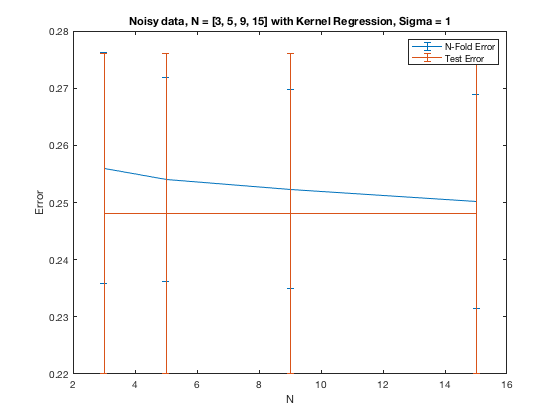
\includegraphics[width=0.6\textwidth]{214.png}
          \caption{Figure on noisy data with Kernel Regression.}
          \label{fig:214}
        \end{figure}
    \end{enumerate}
    Based on these charts, the trend is that test error always stays the same while N-Fold error converges as the number of iterations increases.\\
    \item For both the original data and the noisy, compute both the 10-fold cross validation error on the training set and the test error for K-NN with $K \in \{1,3,4,6,9,14,22,35\}$ and for Kernel Regression with $\sigma \in \{1,3,5,7,9,11\}$.
    \begin{enumerate}
      \item Figure on original data with KNN.\\ \\
        Please see Figure \ref{fig:221}. \\
        \begin{figure}[H]
          \centering
          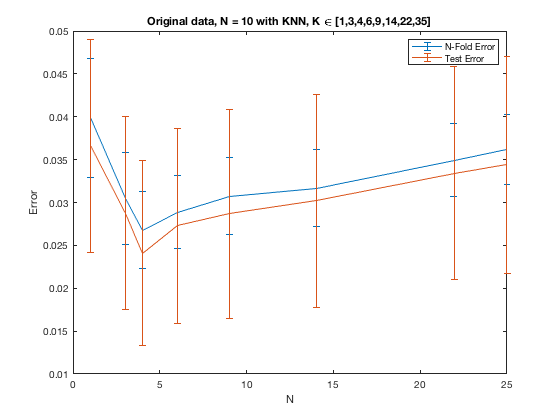
\includegraphics[width=0.6\textwidth]{221.png}
          \caption{Figure on original data with KNN.}
          \label{fig:221}
        \end{figure}
        \item Figure on noisy data with KNN.\\ \\
        Please see Figure \ref{fig:222}. \\
        \begin{figure}[H]
          \centering
          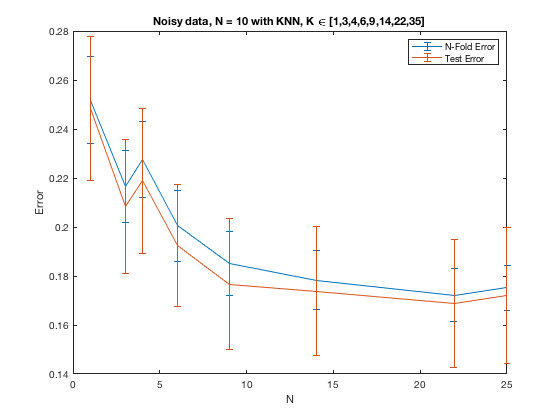
\includegraphics[width=0.6\textwidth]{222.png}
          \caption{Figure on noisy data with KNN.}
          \label{fig:222}
        \end{figure}
        \item Figure on original data with Kernel Regression.\\ \\
        Please see Figure \ref{fig:223}. \\
        \begin{figure}[H]
          \centering
          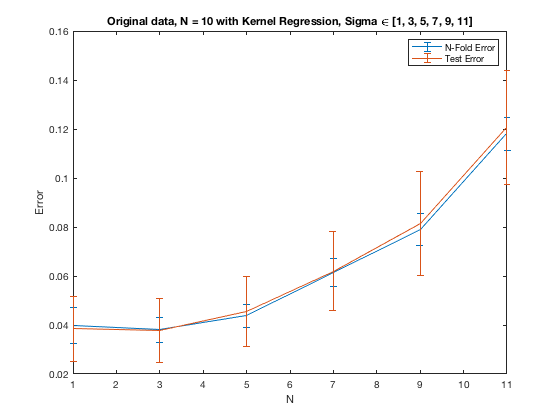
\includegraphics[width=0.6\textwidth]{223.png}
          \caption{Figure on original data with Kernel Regression.}
          \label{fig:223}
        \end{figure}
        \item Figure on noisy data with Kernel Regression.\\ \\
        Please see Figure \ref{fig:224}. \\
        \begin{figure}[H]
          \centering
          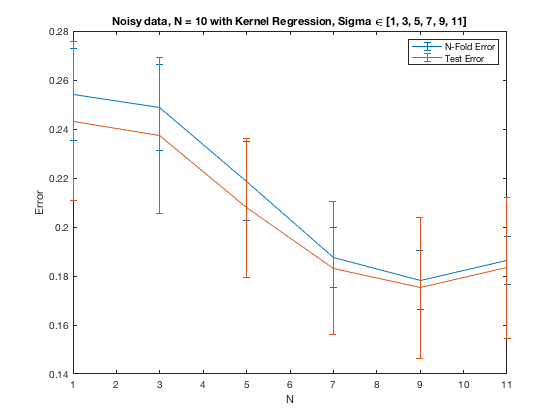
\includegraphics[width=0.6\textwidth]{224.png}
          \caption{Figure on noisy data with Kernel Regression.}
          \label{fig:224}
        \end{figure}
    \end{enumerate}
    Based on these charts, the best $K$ is 4 for original data, 3 for noisy data. The best $\sigma$ is 3 for original data, 9 for noisy data.\\

    \section{Logistic Regression}

    For the code part, please see \path{gradient_ascent_fixed.m}, \path{gradient_ascent_decay.m}, \path{logistic_regression.m} and \path{logistic_xval_error.m}.\\
    \begin{enumerate}
      \item Implement gradient ascent with step size that decays over time.
      \begin{enumerate}
        \item Figure on original data.\\ \\
        Please see Figure \ref{fig:311}. \\
        \begin{figure}[H]
          \centering
          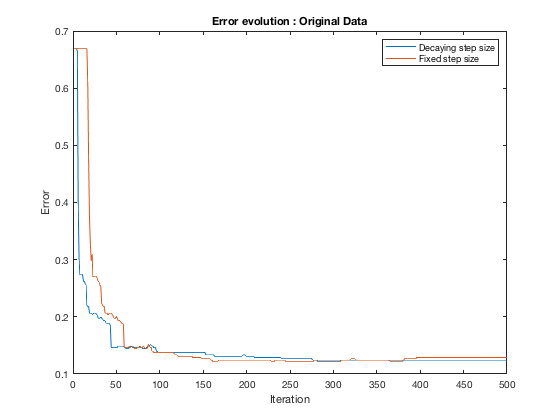
\includegraphics[width=0.6\textwidth]{311.png}
          \caption{Figure on original data.}
          \label{fig:311}
        \end{figure}
        \item Figure on noisy data.\\ \\
        Please see Figure \ref{fig:312}. \\
        \begin{figure}[H]
          \centering
          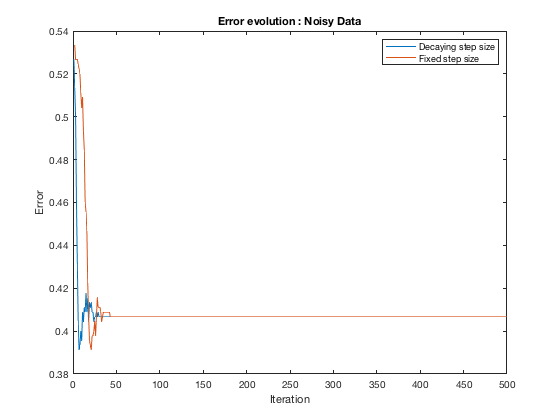
\includegraphics[width=0.6\textwidth]{312.png}
          \caption{Figure on noisy data.}
          \label{fig:312}
        \end{figure}
      \end{enumerate}
      There is an improvement because with both step size being 0.0001, the error gradient ascent with step size that decays over time will continue to decrease if we run more steps. Gradient ascent with a step size that decays over time will converge to the optimal value faster than gradient ascent with a step size that is small enough. \\

      \item Add an extra feature to your data that is always set to 1, and perform gradient ascent on this new data.
      \begin{enumerate}
        \item Figure on original data.\\ \\
        Please see Figure \ref{fig:321}. \\
        \begin{figure}[H]
          \centering
          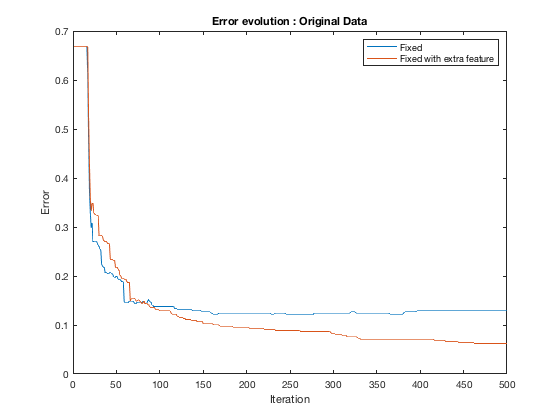
\includegraphics[width=0.6\textwidth]{321.png}
          \caption{Figure on original data.}
          \label{fig:321}
        \end{figure}
        \item Figure on noisy data.\\ \\
        Please see Figure \ref{fig:322}. \\
        \begin{figure}[H]
          \centering
          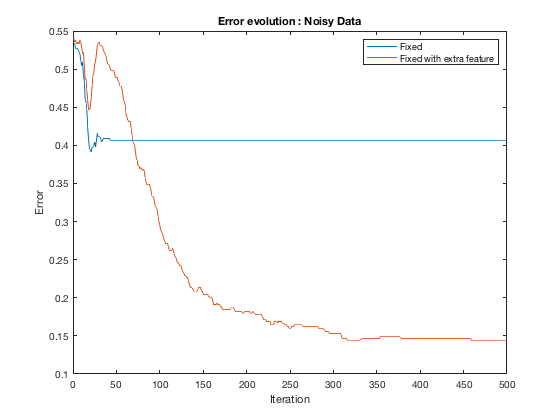
\includegraphics[width=0.6\textwidth]{322.png}
          \caption{Figure on noisy data.}
          \label{fig:322}
        \end{figure}
      \end{enumerate}

      There is an improvement because with this extra feature added, gradient ascent now can converge to a lower error value compared to when it was run on the old data. By adding a constant to the scores, it allows the gradient ascent to shift in the direction that will fit the optimal value better.\\

      \item Implement \path{logistic_regression.m} and \path{logistic_xval_error.m}. For both the original data and the noisy, compute both the $N$-fold error on the training set, for $N = \{3,5,9,15\}$, and the test error.
      \begin{enumerate}
        \item Figure on original data.\\ \\
        Please see Figure \ref{fig:331}. \\
        \begin{figure}[H]
          \centering
          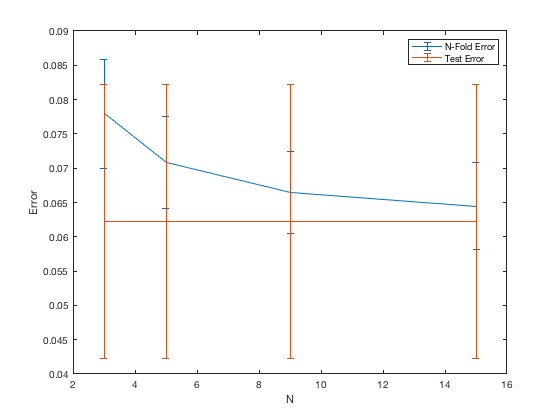
\includegraphics[width=0.6\textwidth]{331.png}
          \caption{Figure on original data.}
          \label{fig:331}
        \end{figure}
        \item Figure on noisy data.\\ \\
        Please see Figure \ref{fig:332}. \\
        \begin{figure}[H]
          \centering
          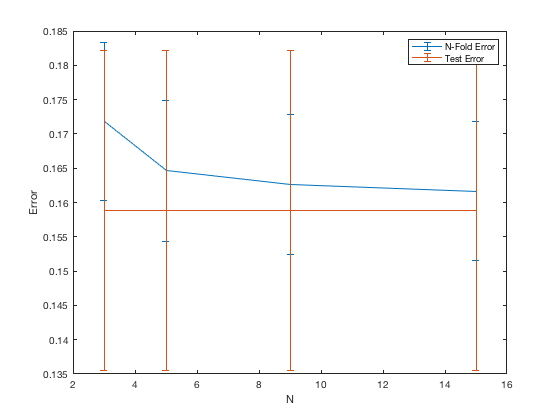
\includegraphics[width=0.6\textwidth]{332.png}
          \caption{Figure on noisy data.}
          \label{fig:332}
        \end{figure}
      \end{enumerate}

    \end{enumerate}

\end{enumerate}

\end{document}